\section{The two cost laws: a line and a staircase}
\label{sec:laws}

\subsection{Parallel formulation}

Both architectures decode output tokens from the same prompt, but their
costs accumulate differently. For autoregressive decoding, each token
requires one forward pass over the growing KV cache. For block-diffusion
decoding, each canvas of \canvasLength{} tokens is denoised in parallel
through $K$ steps, then the model steps to the next canvas. The two
cost laws are:

\begin{align}
\label{eq:ar}
T_{\textsc{ar}}(L_{\mathrm{out}}) &= \arBase + \arSlope \cdot L_{\mathrm{out}} && \text{(ms, linear)} \\
\label{eq:dg}
T_{\textsc{dg}}(L_{\mathrm{out}}) &= \dgBase + \dgStep \cdot \Bigl(\bigl\lceil \tfrac{L_{\mathrm{out}}}{\canvasLength}\bigr\rceil - 1\Bigr) && \text{(ms, staircase)}
\end{align}

where $L_{\mathrm{out}}$ is the output length in tokens. The two laws
have the same form $T = a + b \cdot f(L)$ but differ in what $a$ and $b$
represent physically:

\begin{itemize}[nosep]
\item \emph{AR:} $a = \arBase$\,ms is the prompt prefill cost
  (amortised by prefix caching across requests). $b = \arSlope$\,ms is
  the per-token decode cost --- one forward pass over the KV cache per
  token. Every additional output token costs exactly $\arSlope$\,ms,
  regardless of position.

\item \emph{DG:} $a = \dgBase$\,ms is the first-canvas cost: prompt
  prefill plus $K{=}8$ denoising steps over \canvasLength{} tokens.
  Because each denoising step re-attends the full prompt, prefill is
  paid $K$ times, making $a$ much larger than AR's. $b = \dgStep$\,ms
  is the marginal cost of one additional canvas --- a fresh denoising
  pass over a new block of \canvasLength{} tokens. Within a canvas, $b
  = 0$: additional tokens are free because they are denoised in
  parallel.
\end{itemize}

The operating point $K{=}8$ was selected as the latency/quality knee:
quality is flat above $K{=}8$ (0.853 at $K{=}8$, 0.858 at $K{=}32$)
while latency saturates above $K{=}16$. Each additional canvas costs
\dgStep\,ms (median of 7 measured transitions, range
\dgStepLo--\dgStepHi).

The key structural difference: within a canvas, DG emits tokens for free
(parallel denoising), while AR pays $\arSlope$\,ms per token. At canvas
boundaries, DG pays a fixed $\dgStep$\,ms step, while AR's cost is
unaffected. The shapes cross where the accumulated per-token cost equals
the staircase floor:
\begin{equation}
\label{eq:lcross}
L^{*} = \frac{\dgBase - \arBase}{\arSlope} = \crossoverL \text{ tokens},
\qquad
\lambda^{*} = \frac{1000}{\dgBase} = \crossoverLambda \text{ events/s}
\end{equation}
where $L^{*}$ is the output length at which the two cost laws produce
equal latency (i.e., $T_{\textsc{ar}}(L^{*}) = T_{\textsc{dg}}(L^{*})$),
and $\lambda^{*}$ is the maximum serial event rate before a queue
forms (the reciprocal of the DG base, in events per second). Below
$L^{*}$, AR is cheaper; above it, DG is --- until the next canvas edge,
where the gap widens again.

\begin{figure}[t]
\centering
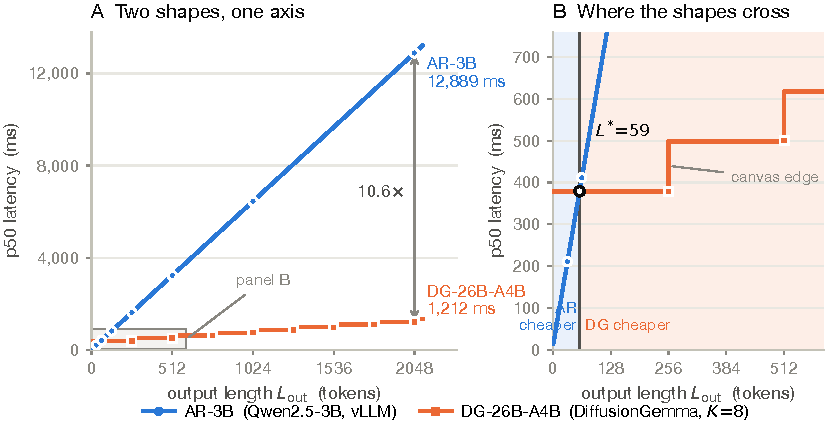
\includegraphics[width=\linewidth]{figures/fig1_cost_shapes.pdf}
\caption{The two cost shapes as a grouped bar chart (BGL, $n{=}200$,
$K{=}8$). AR latency grows linearly; DG latency grows as a staircase.
The gap widens from $4.3\times$ at $L{=}256$ to $10.6\times$ at
$L{=}2048$.}
\label{fig:shapes}
\end{figure}

\begin{figure}[t]
\centering
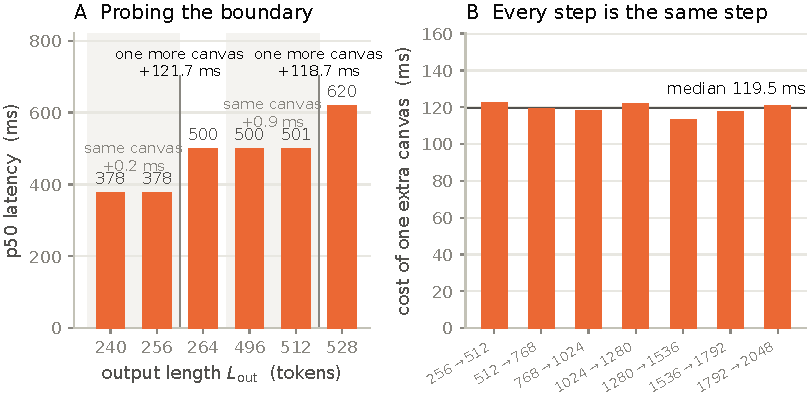
\includegraphics[width=\linewidth]{figures/fig2_canvas_edges.pdf}
\caption{The staircase probed ($K{=}8$, BGL, $n{=}200$).
\textbf{A:} latency is flat inside a canvas and jumps at the boundary.
\textbf{B:} all seven canvas transitions out to $L{=}2048$ cost the same
within run-to-run noise (range \dgStepLo--\dgStepHi\,ms, median \dgStep\,ms).}
\label{fig:edges}
\end{figure}

\subsection{What the base is made of}

The \dgBase\,ms base is 37--53\% prefill (by linear interpolation
between $K{=}2$ and $K{=}8$; see Appendix~\ref{app:decomp}). Each
denoising step re-attends the full prompt, so prefill is paid $K$ times.
If the prompt KV were cached across denoising steps, the base could fall
toward $\sim$150\,ms and $L^{*}$ would move downward. We treat the
measured base as the operative number; see Appendix~\ref{app:forced} for
the asymmetry with the batching caveat.

\subsection{Generalisation}

Both laws generalise from BGL to HDFS within 1.7\%. The AR p50 at
$L{=}\canvasLength$ moves from \arBgl\,ms to \arHdfs\,ms ($+0.03\%$); the
diffusion canvas step moves from \bglStep\,ms to \hdfsStep\,ms ($+1.7\%$).
